\section{Zielsetzung}
Das Ziel des vorliegenden Versuches ist es das Energiespektrum des Krebnebels aus den rekonstruierten Ereignissen zu bestimmen. Dazu wird mit Hilfe von Entfaltungsmethoden aus den gemessenen Energien und den Detektoreigenschaften das ursprünglich emittierte Spektrum bestimmt.
\section{Theorie}
In der Astroteilchenphysik werden die sogenannten Botenteilchen, die von Quellen ausgesendet werden, in drei Kategorien eingeteilt. Die geladene kosmische Strahlung wird durch Magnetfelder im intergalaktischen und interstellarem Medium abgelenkt. Deshalb lässt sich zwar bedingt auf ihre Ladung zurückschließen, aber die Richtungsinformation zu ihrer Quelle geht verloren. Eine weitere Kategorie bilden die Neutrinos. Sie sind durch ihren extrem kleinen Wirkungsquerschnitt nur schwer nachzuweisen. Durch ihre neutrale Ladung werden sie jedoch nicht abgelenkt und besitzen somit grundsätzlich eine Richtungsinformation. Die aktuelle Forschung beschäftigt sich mit den ersten Hinweise zu Neutrinopunktquellen. Die dritte Kategorie bilden die hochenergetischen Photonen. Sie übermitteln die Richtungsinformation zu ihrer Quelle und können sowohl direkt mit Sateliten nachgewiesen werden oder mit bodengebundenen Tscherenkow-Teleskopen. Dafür wechselwirken die hochenergetischen Photonen mit der Atmosphäre. Die entstehenden Teilchenkaskaden bewegen sich zum Teil im Medium über Lichtschnell, sodass es zur Abstrahlung von Tscherenkowlicht kommt. Dieses wird von den Teleskopen gemessen. Die Teilchenkaskaden werden jedoch nicht nur durch Photonen, sondern ebenfalls durch geladene Botenteilchen wie zum Beispiel Protonen. Die Abbildung \ref{fig:Boten} zeigt schematisch die drei Arten von Botenteilchen und ihren Weg von der Quelle zur Erde.\\
\begin{figure}
  \centering
  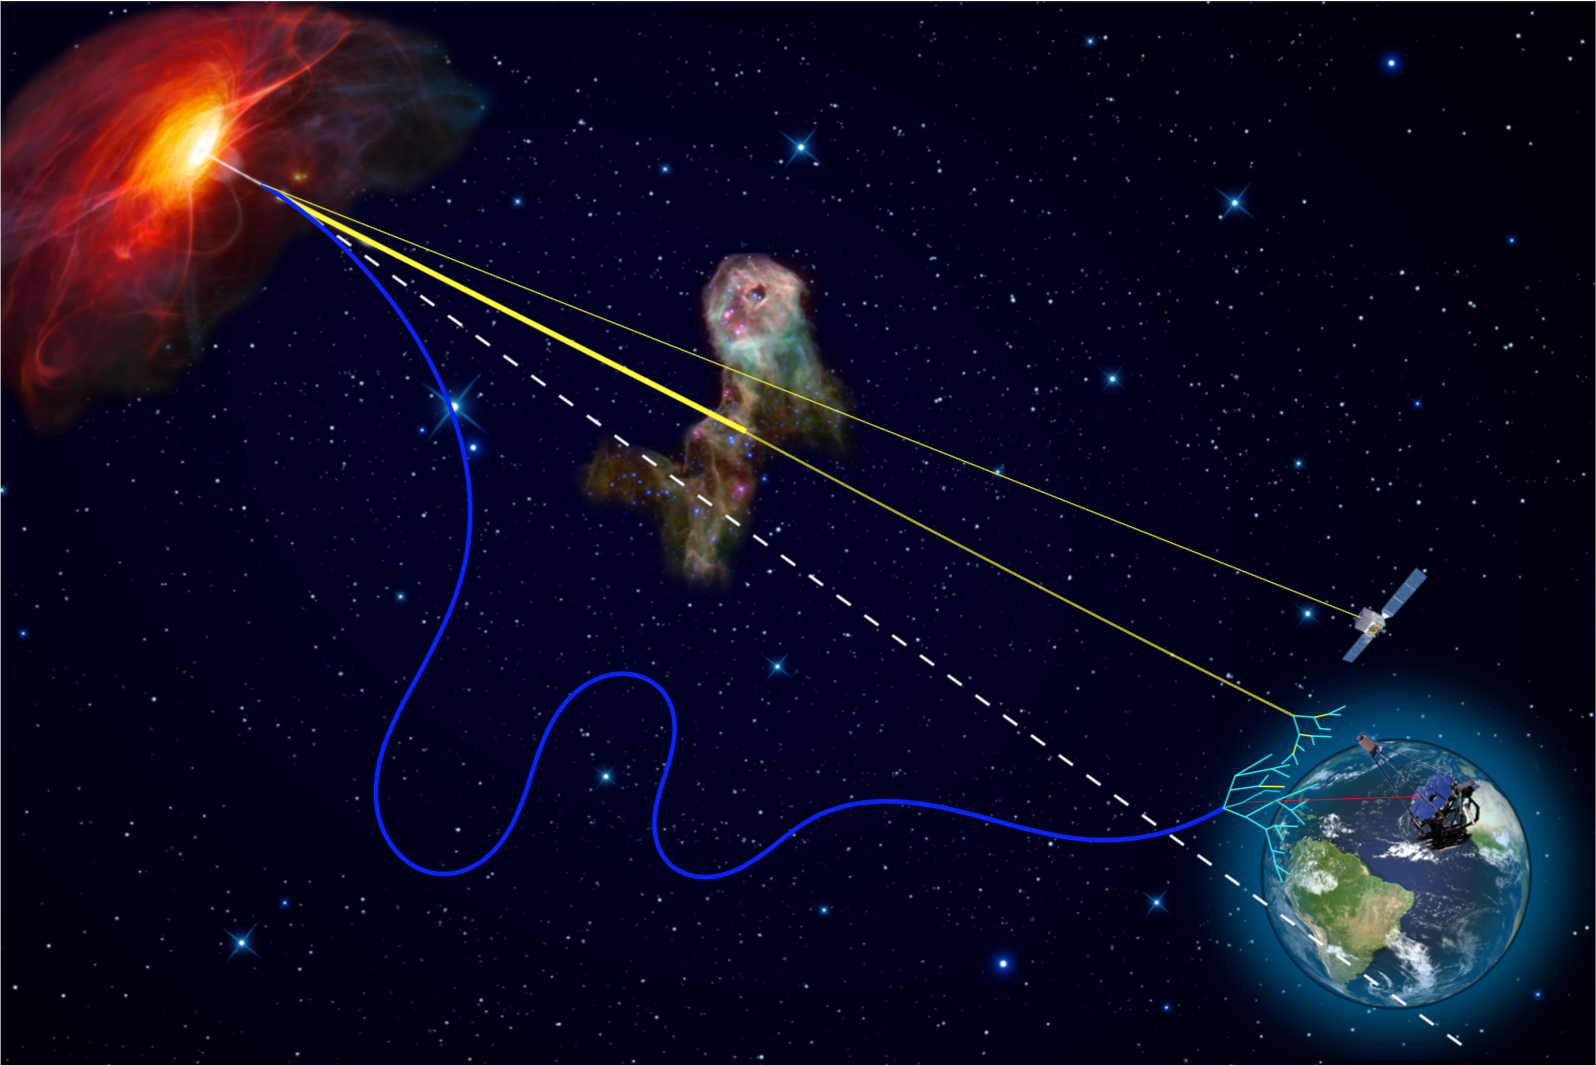
\includegraphics[width=0.6\textwidth]{graphics/Folie5.png}
  \caption{Schematische Darstellung von astrophysikalischen Botenteilchen auf ihrem Weg von der Quelle zur Erde. Die blaue Linie stellt geladene Teilchen dar, die Neutrinos werden durchh die gestrichelte Linie veranschaulicht und die Photonen durch die gelbe.\cite{anleitung}}
  \label{fig:Boten}
\end{figure}
Der vorliegende Versuch beschäftigt sich mit der Gammaastronomie und somit den Photonen als Botenteilchen.
\subsection{FACT}
Das \textit{First G-APD Cherenkov Telescope}, \cite{Anderhub_2013} kurz FACT, ist ein bodengebundenes, abbildendes Tscherenkow-Teleskope. Ein Foto von FACT ist in Abbildung \ref{fig:FACT} zu sehen. Auf Grund der geringeren Luftverschmutzung steht es im Obersatorio del Roque de los Muchachos auf La Palma. Dort operiert es seit 2011, ist seit 2012 ferngesteuert und seit 2017 operiert es robotisch. FACT ist ein Forschungsteleskop der Gammaastronomie, dessen Ziel ist eine neue Detektortechnologie zu testen. Es werden siliziumbasierte Halbleiterphotodetektoren verwendet, weil (???). Dies ermöglicht eine möglichst lückenlose Überwachung von Gammastrahlungsquellen, wie dem Supernovaüberrest Krebsnebel oder extragalaktischen Quellen, den Blazaren.
\begin{figure}
  \centering
  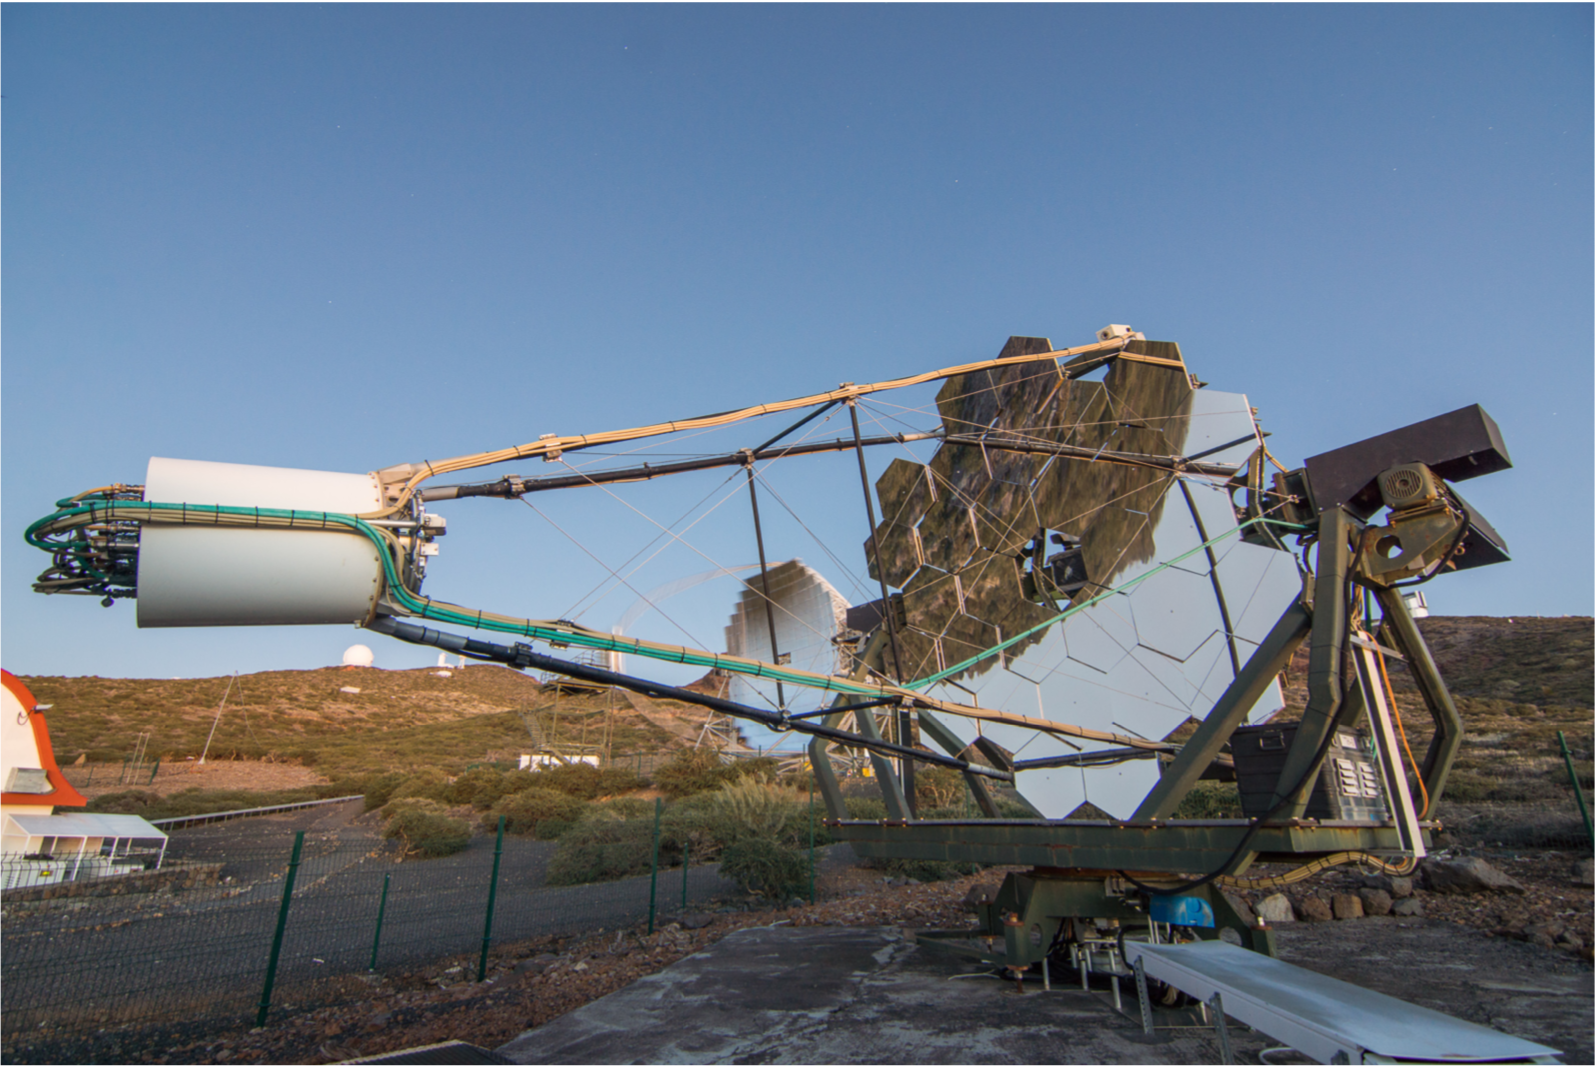
\includegraphics[width=0.8\textwidth]{graphics/Max.png}
  \caption{ FACT im Observatorio del Roque de los Muchachos, La Palma, Spanien. Im Hintergrund ist das MAGIC-1 Teleskop und das William-Herschel-Telescope zu sehen. [M. Nöthe, 2018]}
  \label{fig:FACT}
\end{figure}
\subsection{Entfaltung}
In der Astrophysik muss in der Regel aus Ladungsdepositionen im Detektor auf die ursprünglichen Eigenschaften der Teilchen zurückgeschlossen werden. Eine Möglichkeit dafür stellt die Entfalltung dar.\\
Das \textit{inverse Problem} bezeichnet dabei den Vorgang von der Verteilung der gemessenen Größen auf die physikalischen zu schließen. Das inverse Problem lässt sich durch die Fredholmsche-Integralgleichung erster Art darstellen:
\begin{align}
	g(y)=\int A(y,x)f(x)\text{d}x + b(y)
	\label{eqn:1}
\end{align}
Die gesuchte Wahrscheinlichkeitsdichte ist dabei $f(x)$ in Abhängigkeit von der Größe $x$, $g(y)$ widerum beschreibt die Wahrscheinlichkeitsdichte in Abhängigkeit der gemessenen Größen $y$. Der Untergrund wird durch $b(y)$ beschrieben und $A(y,x)$ stellt den Faltungskern dar. Dieser wird benötigt um den Detektor und damit den Zusammenhang zwischen der gemessenen Größe $y$ und der physikalischen Größe $x$ zu beschreiben. \\
Um die physikalischen Größen zu erhalten, muss \eqref{eqn:1} invertiert werden. Dazu werden die kontinuierlichen Wahrscheinlichkeitsdichten zunächst diskretisiert. Dadurch entsprechen sie einem Histogram der jeweiligen Größe und \eqref{eqn:1} lässt sich darstellen mit:
\begin{align}
	\vec{g} = \pmb{A}\vec{f} + \vec{b}
\end{align}
Der $M$-dimensionale Vektor $\vec{g}$ steht für das Histogramm der geschätzten Gamma-Energien für alle gemessenen Photonen. Der ebenfalls $M$-dimensionale Vektor $\vec{b}$ beschreibt das Untergrundhistogram und lässt sich aus den Off-Messungen ableiten. Der $N$-dimensionale Vektor $\vec{f}$ beschreibt die wahren Gamma-Energien und die $M\times N$-dimensionale Matrix $\pmb{A}$ stellt die Migrationsmatrix des Energieschätzers da. \\
Von diesem Punkt aus kann nun der Schätzer $\hat{\vec{f}}$ bestimmt werden. Die Akzeptanzkorrektur kann entweder zuletzt auf den Schätzer $\hat{\vec{f}}$ angewendet werden oder die Migrationsmatrix $\pmb{A}$ muss zu Beginn geeignet normiert werden.
\subsubsection{Naive SVD-Entfaltung}
Die Naive SVD-Entfaltung bildet die einfachste, aber auch fehleranfälligste Möglichkeit einer Entfaltung. Um an die wahre Verteilung $\vec{f}$ zu kommen, wird die Migrationsmatrix des Energieschätzers $\pmb{A}$ invertriert. Bei nicht quadratischen Matrizen wird dazu die Moore-Penrose-Pseudoinverse gebildet.\\
\begin{align}
	\hat{\vec{f}} = \pmb{A}^{+}(\vec{g} - \vec{b})
	\label{eqn:NSVD}
\end{align}
Diese Lösung ist äquivalent zur Methode der kleinsten Quadrate.
\subsubsection{Poisson-Likelihood-Enfaltung}
Die Annahme, dass die Zählraten in $\vec{g}$ poissonverteilt sind, ermöglicht einen Maximum-Likelihood-Fit durchzuführen. Somit gilt für die Wahrscheinlichkeit für einen Messwert $g_{i}$
\begin{align}
	P(g_{i}) &= \mathcal{P}(g_{i},\lambda_{i}) \; \text{mit}\\
	\vec{\lambda} &= \pmb{A} \cdot \vec{f} + \vec{b}
\end{align}
Die Likelihood ergibt sich folglich zu
\begin{align}
	\mathcal{L} = \prod_{i=1}^{M}\mathcal{P}(g_{i},\lambda_{i})
\end{align}
Numerisch ist es jedoch sinnvoller die negative Log-Likelihood zu minimieren
\begin{align}
	- \ln\mathcal{L} = - \sum_{i=1}^{M}\mathcal{P}(g_{i},\lambda_{i}) = \sum_{i=1}^{M}\ln(g_{i}!) - g_{i} \cdot \ln \lambda_{i} +\lambda_{i}
	\label{eqn:loglike}
\end{align}
sodass sich der Schätzer $\vec{f}$ zu:
\begin{align}
	\hat{\vec{f}} = \text{argmin}\left( -\ln(\vec{f}|\pmb{A},\vec{g},\vec{b})\right)
	\label{eqn:fLike}
\end{align}
ergibt.
\section{Datensatz}
Für den durchzuführenden Versuch liegt bereits ein aufbereiteter Datensatz bzw. mehrere im Datenlevel 3 vor.
\begin{itemize}
	\item \textit{open\_crab\_sample\_dl3.hdf5} Messdaten aus \SI{17.7}{\hour} Oberservationszeit des Krebsnebels.
	\item \textit{gamma\_test\_dl3.hdf5} Testdatensatz bestehend aus \SI{70}{\percent} der ursprünglichen simulierten Quell-Gammas.
	\item \textit{gamma\_corsika\_v1.1.2.hdf5} Informationen über alle simulierten Gamma-Luftschauer.
\end{itemize}
Dazu wurden bereits im Vorfeld die drei Eigenschaften \textbf{Teilchenklasse, Energie} und \textbf{Herkunftsrichtung} der ursprünglichen Teilchen aus den von FACT aufgenommenen Schauer-Ereignissen rekonstruiert. \\
Um dies zu ermöglichen werden die Daten zunächst mit den \textbf{FACT-Tools} \cite{kai_brugge_2018_2386762} analysiert. Dabei wird zunächst die Spannungszeitreihe von jedem Pixel kalibriert und anschließend die Anzahl der Photonen und deren mittlere Ankunftszeit in jedem Pixel ermittelt. Aus diesen werden nun die Pixel ausgewählt, die ein Tscherenkow-Signal enthalten. Zuletzt erfolgt die Parametrisierung des Schauerbildes mit Hilfe der Hillas-Parameter. Diese sind in Abbildung \ref{fig:Para} dargestellt.
\begin{figure}
	\centering
	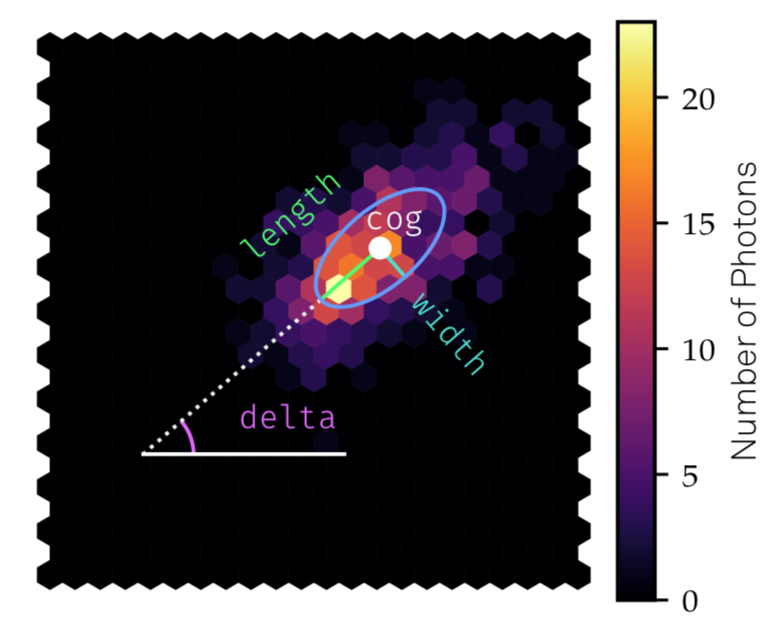
\includegraphics[width=0.6\textwidth]{graphics/Hillas.png}
	\caption{Schauerbild eines Photons mit  den wichtigstens Hillas-Parametern. Der Mittelpunkt wird als \textit{cog} bezeichnet, die beiden Standardabweichungen \textit{length} und \textit{width} stammen aus der Hauptkomponentenanalyse der 2d-Lichtverteilung. Die Orientierung der Hauptachse des Schauers wird mit dem Winkel \textit{delta} zur x-Achse angegeben.\cite{anleitung}}
	\label{fig:Para}
\end{figure}
Anschließend werden Methoden des Maschinellen Lernens verwendet, um die Teilcheneigenschaften zu bestimmen. Dazu werden zunächst Simulationen für einen Testdatensatz durchgeführt, aus diesem lässt sich ebenfalls die Detektorakzeptanz bestimmen. \\
Mit dem Programm \textbf{CORSIKA} \cite{1998cmcc.book.....H} lässt sich sich Produktion der Luftschauer und das anschließend entstehende Tscherenkowlicht, das den Detektor erreicht simulieren. Dafür werden als Eingabewerte die Eigenschaften des Primärteilchens genutzt. Mit dem Programm \textbf{CERES} lässt sich anschließend das FACT-Teleskop simulieren. Dabei werden nicht nur Eigenschaften wie die Spiegel und Kamera-Elektronik beachtet, sondern die Daten am Ende im selben Datenformat wie die eigentlichen Messdaten gespeichert. Der entscheidende Unterschied ist, dass die Informationen über das Primärteilchen erhalten sind.\\
Um zusätzlich den Untergrund abschätzen zu können, werden drei Datensätze simuliert.
\begin{itemize}
	\item Gammas, aus einer punktförmigen Quelle, die im Wobble-Modus beobachtet wird
	\item Gammas, die diffus aus zufälligen Orten im Blickfeld des Teleskop kommen
	\item Protonen, die diffus aus zufälligen Orten im Blickfeld des Teleskop kommen
\end{itemize}
Die Teilchenart wird mithilfe eines Random Forest Klassifikator bestimmt, dieser wurde darauf trainiert diffuse Gammas von den Protonen zu unterscheiden. Der Energieschätzer ist ein Random Forest Regressor, der die Quellgammas als Trainingsdaten nutzt. Die Richtungsrekonstruktion wurde mithilfe der \textit{disp}-Methode durchgeführt. Die eigentlich 2d-Regression für den Herkunftsort der Teilchen reduziert sich dabei auf eine 1-dimensionale unter der Annahme, dass die Quelle auf der Hauptachse vom Schwerpunkt des Schauers liegt. Zudem erhält man eine binäre Klassifikation in welche der beiden möglichen Richtungen auf der Hauptache die Quelle liegt.\\
Aus dieser Analyse entstehen die oben aufgeführten Datensätze, die unter \cite{FACTdata} heruntergeladen werden können.
